%!TEX root = pset2.tex

\section{Titanic Data}\label{sec:tinanic}

\subsection{Logistic Regression}
We use Logistic Regression classifier on the Titanic data to make predictions on survivor results. First, we scale the features so that each one is within the $[0, 1]$ range. 

With no regularization, we obtain a testing set accuracy of $78.31\%$. To find the best $\lambda$, we use the cross validation technique. The validation set accuracy with respect to $\lambda$ is presented in Figure \ref{3_LR_cv}. We therefore choose $\lambda = 10^{-1} = 0.1$ based on the validation accuracy. The test set accuracy is then $76.19\%$. Unfortunately this is not as good as the non-regularized logistic regression on the Titanic data.

\begin{figure}[hb]
\centering
	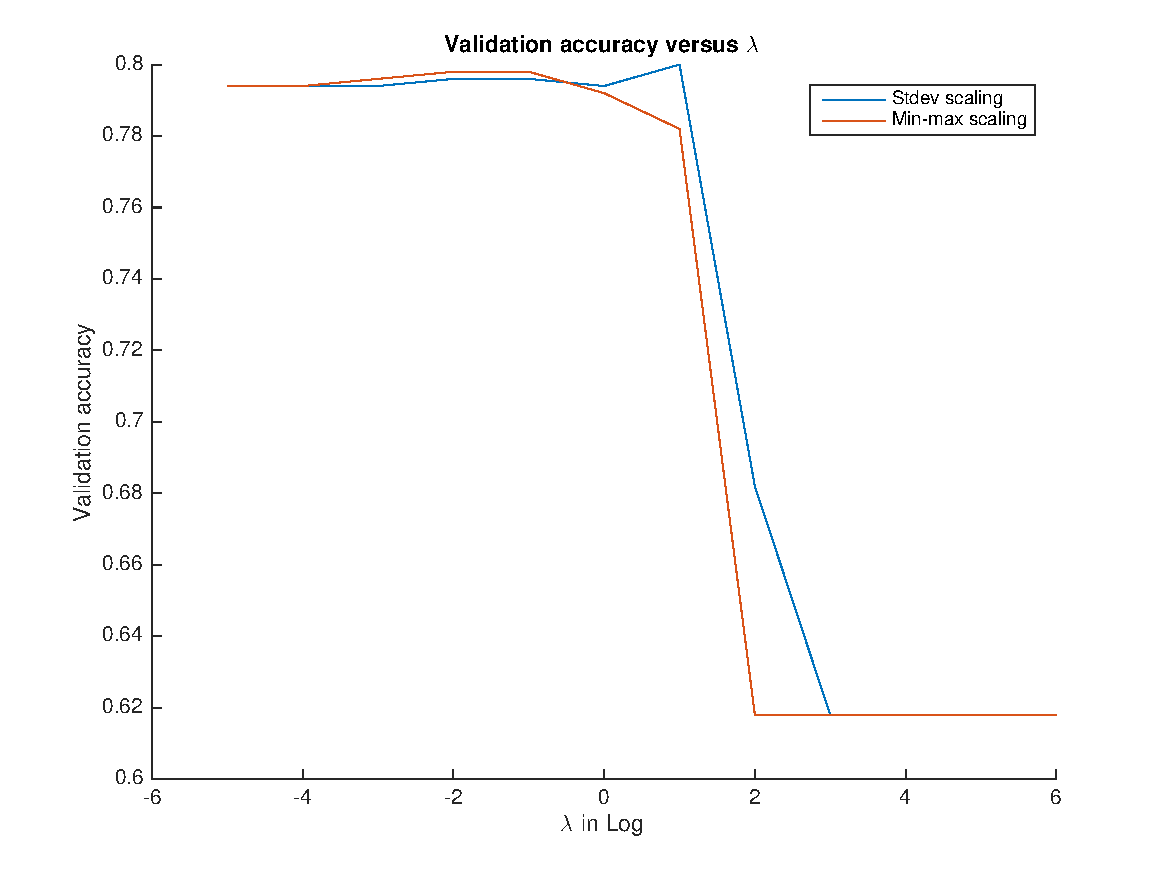
\includegraphics[scale=0.6]{hw2_3_cv.pdf}
	\caption{Tinanic Data, Cross validation error in logistic regression with respect to $\lambda$}\label{fig:3_LR_cv}
\end{figure}
